\chapter{Исследовательская часть}

\section{Технические характеристики}

Технические характеристики устройства,на котором проводились замеры:

\begin{itemize}
	\item Процессор: AMD Ryzen 7 5800H (16) @ 4.46 ГГц;
	\item Оперативная память: 16 ГБ;
	\item Операционная система: Arch Linux x86\_64.
\end{itemize}

При проведении замеров ноутбук был включён в сеть и были запущены только системные приложения и jupyter notebook.

\section{Временные характеристики}
В таблице (\ref{tbl:time_algo}) приведены временные характеристики, полученные в результате замеров времени алгоритмов (\ref{recursive-levenshtein}) и (\ref{cache-levenshtein}). Для каждой длины замер проводился 100 раз, при этом для каждой итерации создавались 2 случайные строки заданной длины и использовались как аргументы к алгоритмам. Итоговое время взято как среднее арифметическое всех полученных замеров.

\begin{table}[ht]
	\small
	\begin{center}
		\begin{threeparttable}
			\caption{Временные характеристики}
			\label{tbl:time_algo}
			\begin{tabular}{|r|r|r|}
				\hline
				Длина строки, символы & Рекурсивный алгоритм, мкс & Итерационный алгоритм с кешем, мкс \\
				\hline
				2 & \text{151}  & 98  \\
				\hline
				3 & \text{452}  & 99  \\
				\hline
				4 & \text{1 540}  & 120  \\
				\hline
				5 & \text{7 077}  & 138  \\
				\hline
				6 & \text{29 669}  & 155  \\
				\hline
				7 & \text{138 545}  & 177  \\
				\hline
				8 & \text{658 211}  & 203  \\
				\hline
				9 & \text{2 952 534}  & 223  \\
				\hline
				10 & \text{20 510 843}  & 245  \\
				\hline
			\end{tabular}	
		\end{threeparttable}
	\end{center}
\end{table}

Полученные замеры также можно увидеть на графике (\ref{fig:time_graph}):

\begin{figure}
	\centering
	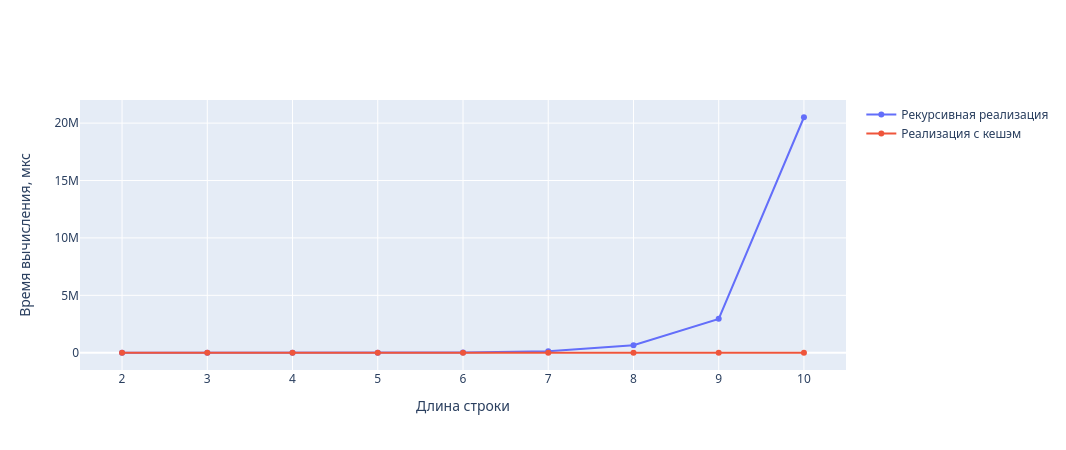
\includegraphics[width=0.9\textwidth]{time}
	\caption{График зависимости времени работы алгоритмов от длины строк}
	\label{fig:time_graph}
\end{figure}

Как видно из таблицы (\ref{tbl:time_algo}) и графика (\ref{fig:time_graph}), рекурсивный алгоритм существенно уступает итерационному по временным характеристикам.

\pagebreak

\section{Ёмкостные характеристики}

В таблице (\ref{tbl:mem_algo}) приведены временные характеристики, полученные в результате замеров памяти алгоритмов (\ref{recursive-levenshtein}) и (\ref{cache-levenshtein}) с помощью модуля tracemalloc. Так как для рекурсивной реализации размер выделяемой памяти существенно зависит от глубины рекурсии, то есть от входных строк, то для каждой длины строки для рекурсивного алгоритма алгоритм был проведён 10 раз на случайных строках. Для итерационного алгоритма выделяемая память не зависит от входных строк(при одинаковой длине), так как размер матрицы кеша зависит только от размеров строк. За характеристику памяти взята пиковая память, то есть максимальный объём памяти выделенный функции во время её выполнения.


\begin{table}[ht]
	\small
	\begin{center}
		\begin{threeparttable}
			\caption{Временные характеристики}
			\label{tbl:mem_algo}
			\begin{tabular}{|r|r|r|}
				\hline
				Длина строки, символы & Рекурсивный алгоритм, байты & Итерационный алгоритм с кешем, байты \\
				\hline
				2 & 48  & 232  \\
				\hline
				3 & 247  & 288  \\
				\hline
				4 & 288  & 392  \\
				\hline
				5 & 312  & 480  \\
				\hline
				6 & 404  & 584  \\
				\hline
				7 & 498  & 704  \\
				\hline
				8 & 674  & 904  \\
				\hline
				9 & 1 429  & 1 056  \\
				\hline
				10 & 2 201  & 1 224  \\
				\hline
			\end{tabular}	
		\end{threeparttable}
	\end{center}
\end{table}

Также зависимость из таблицы отражена на графике (\ref{fig:mem_graph}).

Как видно из графика (\ref{fig:mem_graph}) и таблицы (\ref{tbl:mem_algo}), при небольших размерах строки рекурсивная реализация выигрывает итерационную, одна начиная с длин строк 9, вариант с кешем становится эффективнее, так как реализация рекурсии требует больший объем памяти под входные строки и вызовы.
\begin{figure}
	\centering
	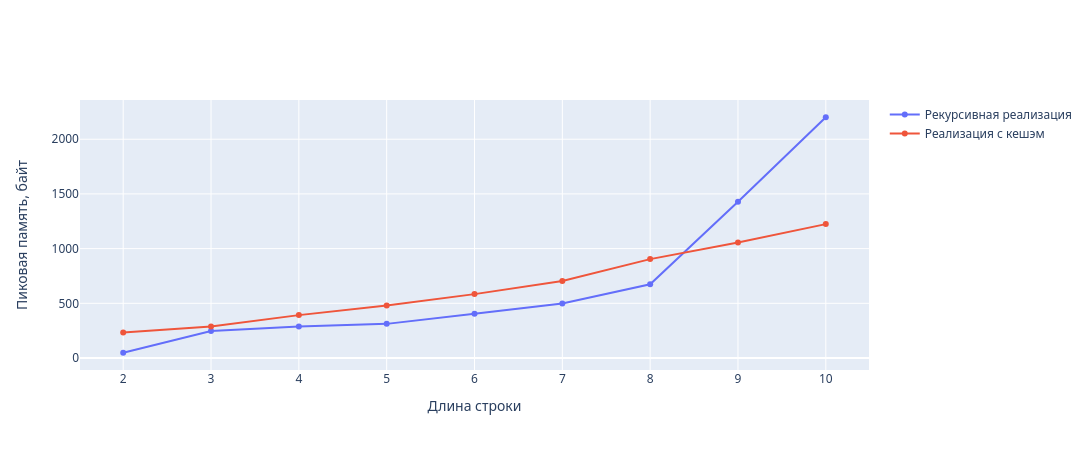
\includegraphics[width=0.9\textwidth]{memory}
	\caption{График зависимости требуемой памяти для работы алгоритмов от длины входных строк}
	\label{fig:mem_graph}
\end{figure}

\pagebreak

\section{Вывод}

В данном разделе было проведено исследование временных и ёмкостных характеристик алгоритмов рекурсивного поиска расстояния Левенштейна и итерационного поиска расстояние Левенштейна с кешем.

По результатам исследования оказалось, что рекурсивная реализация существенно проигрывает итерационной по времени. Что касается ёмкостных характеристик, то при длине входных строк $\leq$ 8 рекурсивная реализация эффективная, однако при длине $\geq$ 9 эффективнее становится итерационный вариант из–за того, что рекурсивный алгоритм делает много вызовов функции.

\clearpage
